\documentclass[11pt]{article}
\usepackage[utf8]{inputenc}
\usepackage{graphicx}
\usepackage{amsmath}
\usepackage{hyperref}
\usepackage{geometry}
\usepackage{multirow}
\usepackage{natbib}

\geometry{
 left=25mm,
 right=25mm,
 top=25mm,
 bottom=25mm
}

\setlength{\columnsep}{10mm}

\hyphenpenalty=1000
\tolerance=2000
\sloppy

\title{Intel Image Classification}
\author{Anahit (Ana) Hovhannisyan, Jesse Keller, Roxy Rong}
\date{MIDS 281, Section 3, Fall 2023}

\begin{document}

\maketitle
\begin{abstract}%
In this project, we present a comprehensive study on classifying urban and rural snapshot photos using a combination of advanced feature extraction techniques and machine learning models. Utilizing a dataset of approximately 16,000 labeled images, we explore various feature vectors including color features, frequency features, edge detection, Histogram of Oriented Gradients (HOG), Bag of Visual Words (BOVW), and features extracted from the pre-trained VGG16 neural network. We apply Principal Component Analysis (PCA) for dimensionality reduction and employ logistic regression, support vector machine, and random forest classifiers for image classification. Our study includes an in-depth analysis of hyperparameter tuning, model efficiency, and accuracy. We emerge with a single model based on a logistic regression classifier that provided excellent results in both efficiency and accuracy while outperforming alternative classifiers. 
\end{abstract}

\section{Introduction}

Our project's objective is to classify urban and rural snapshot photos into one of six categories, catering to both commercial and non-commercial applications. In commercial settings, such as photo-sharing mobile applications, it enables automatic organization and simplified browsing of images. For non-commercial uses, it serves in intelligence gathering and automatic copyright infringement detection.

\begin{figure*}[h!]
\centering
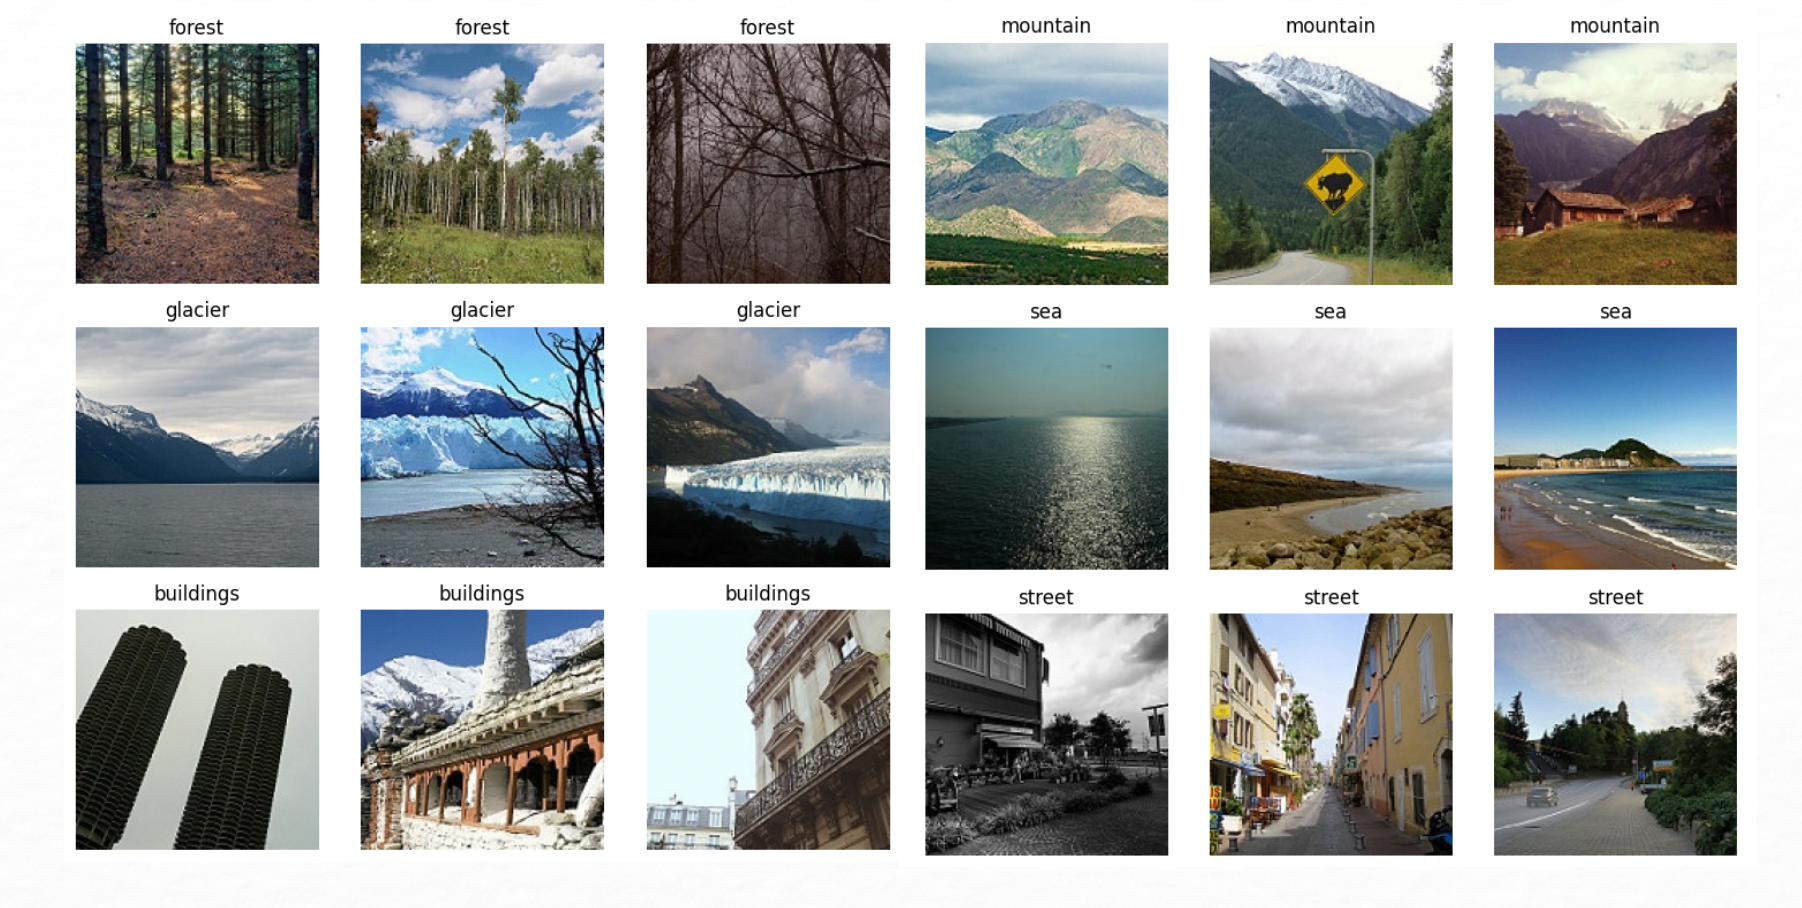
\includegraphics[width=0.8\textwidth]{sample_category.png}
\caption{Three images per class are shown.}
\label{fig:sample categories}
\end{figure*}

\section{Dataset}
Our dataset is available via Kaggle and is a publicly available set of approximately 16,000 labeled snapshots assembled by Puneet Bansal and provided by Intel\cite{IntelImageDataset}. No category is disproportionately over or under represented. The data set is divided into 10,786 images for training, 2,672 images for validation of the models and 2,853 images for testing. Example images are shown in Figure \ref{fig:sample categories}. 

No pre\-processing of the images is conducted. However, monochromatic images and those that are not exactly 150x150 pixels are removed from the datasets to standardize the samples.

\begin{table*}[h]
\centering
\begin{tabular}{|c|c|c|c|c|}
\hline
\textbf{Category} & \textbf{Total} & \textbf{Partial Resolution} & \textbf{Monochrome} & \textbf{FullSize And Color} \\ \hline
buildings         & 2191          & 1                          & 94                  & 2190                        \\ \hline
forest            & 2271          & 8                          & 68                  & 2263                        \\ \hline
glacier           & 2404          & 17                         & 20                  & 2387                        \\ \hline
mountain          & 2512          & 17                         & 22                  & 2495                        \\ \hline
sea               & 2274          & 4                          & 82                  & 2270                        \\ \hline
street            & 2382          & 1                          & 330                 & 2381                        \\ \hline
\textbf{Total}    & \textbf{14034}& \textbf{48}                & \textbf{616}        & \textbf{13986}              \\ \hline
\end{tabular}
\caption{Sample counts for images included per category, including total image count, partial resolution image count, monochromatic image count, and finally images remaining after standardization.}
\label{table EDA}
\end{table*}

\section{Feature Extraction}
To create an extensive set of feature vectors, various algorithms are utilized. We select algorithms that look at the images at the global level (i.e. color and intensity histograms, along with frequency components), at the object level (edge detectors and bag of visual words), and through the lens of a pre-trained neural network, VGG16. Visualizations of the simple vectors are shown in Figure \ref{fig:features}, A principal component analysis of the set of feature vectors generates a subset of components resulting in a dramatic reduction in dimensionality.

\subsection{Color Feature}
Initial data exploration (see Figure \ref{fig:color_eda}) suggests that color should play an important role in distinguishing images. A vector that contains the mean and standard deviation of the hue, saturation, and intensity channels of each image, as well as the full histogram of the three channels is created. The red, green, and blue channels of the image, when treated the same way, do not provide the same information.

\begin{figure}[h!]
\centering
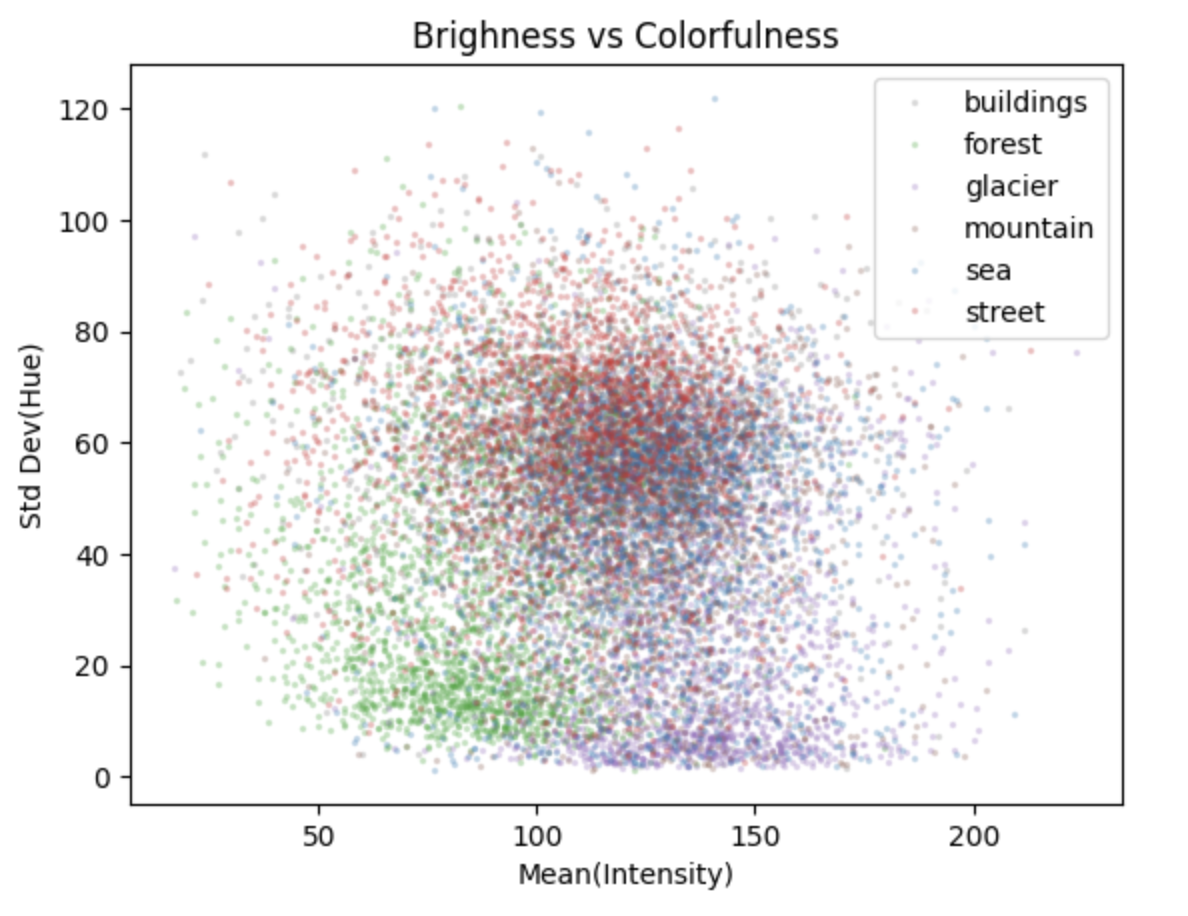
\includegraphics[width=0.7\textwidth]{color_eda.png}
\caption{Data Exploration of the relationship between hue distribution and mean intensity.}
\label{fig:color_eda}
\end{figure}

\subsection{Frequency Feature}
Each image is Fourier transformed to extract frequency data. Windowing is conducted to reduce artifacts from harsh image edges which are not continuous. The frequency data is used to distinguish between repeating mid-frequency elements like trees or windows on buildings, images with significant low-frequency data like oceans or skies, or high-frequency data like crevices in mountains or glaciers.

\subsection{Edge Feature}
Two edge detection techniques are utilized in an attempt to extract more information about objects in each image: Canny\cite{Canny1986} and Holistically-Nested Edge Detection (“HED”)\cite{XieTu2015}. Canny is a non-heuristic algorithm that uses a combination of Gaussian blurs, gradient detection, and hysteresis to create connected edges. HED is a computationally intensive, learning-based end-to-end edge detection pipeline trained on existing images. Both algorithms provide clear shapes to the human eye, with HED providing obvious features like cars, people, and buildings. However, it is challenging to extract a meaningful feature vector from the data as there is very little correlation between the locations of edges between images. For example, identical images that are shifted by 1 pixel would return feature vectors with few elements in common. Treating the entire image as a feature vector does not provide any significant benefit, so feature vectors depending on the location of edges are not included in our model.

\subsection{Histogram of Gradients(HOG)}
We generate a feature vector containing the results of the Histogram of Gradients (HOG) algorithm\cite{DalalTriggs2005}. A cell size of 15 evenly maps over the 150x150 pixel images. Given that HOG is used to extract the directionality of features and their location in the image, we choose this feature to identify vertical or horizontal images in the natural and urban scenes in the dataset. For example, an ocean has a strong horizontal component in the middle of the image. A building has few vertical and no horizontal components at the top of the image. A directionality of 8 detects the horizontal and vertical features of seas and buildings as well as diagonal features found in mountains and glaciers. 

\begin{figure*}[h!]
\centering
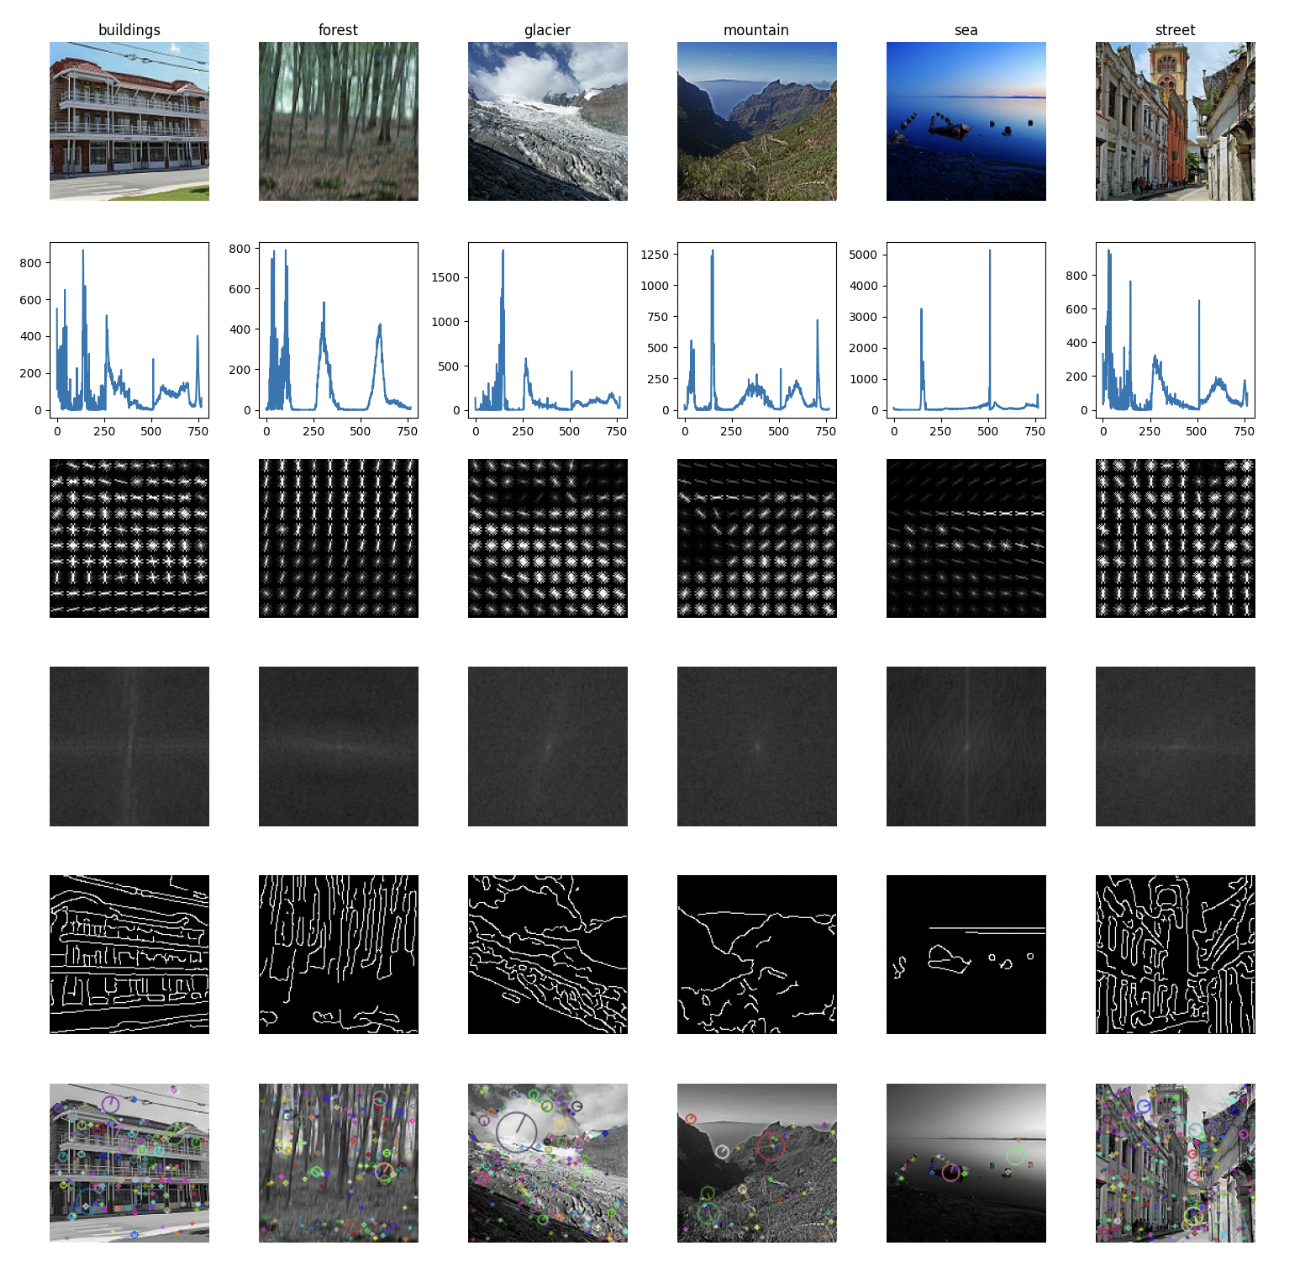
\includegraphics[width=0.9\textwidth]{features.png}
\caption{Visualization of feature vectors for some representative images. From top to bottom: sample image, HSV histogram, HOG render, Fourier transform, Canny edge detection, and Bag Of Visual Words descriptors
}
\label{fig:features}
\end{figure*}

\subsection{Bag of Visual Words (BOVW)}
We utilize the SIFT algorithm\cite{Lowe1999} to pick out significant corner features from a random selection of 20\% of our training images. SIFT is great as it is invariant to scale, rotation, translation, illumination, and blur. Following previous work with a similar size dataset and number of categories, we set k value at 200 in the k-means clustering step to generate a pool of common visual features. We then apply TF-IDF to compute an optimal codebook for the Bag Of Visual Words algorithm\cite{GidarisEtAl2020}. By counting how often the most significant features appeared in each image, a feature vector is formed. We choose this feature to help identify objects in sample images for improved classification. We hypothesize that any boats captured in an image can point to a “sea” class or trees can point to a “forest” class.

\subsection{VGG16}
We use a convolutional neural network to provide additional semantic information about the image. We utilize the pre-trained VGG16 network\cite{SimonyanZisserman2014} with its default setting implemented by the Python Keras package. VGG16 is trained on the ImageNet database and can distinguish between 1000 different image categories. The fact that VGG16 is trained on millions of images that cover natural and urban scenes gives us good results without any tuning.

\subsection{Feature Vector Future Work}
While the set of feature vectors above generates a good model, two other feature vector techniques should be investigated in the future. The first, Local Binary Patterns\cite{Pietikainen2010}, would likely allow us to identify textures associated with the broken ice of glaciers or the smooth asphalt of streets. While we use the hue and saturation histograms as feature vectors, a more refined approach that identifies the most common or most distinctive colors - a bag of visual colors algorithm - may have higher accuracy at lower dimensionality.


\section{Feature Selection}
\subsection{Principal Component Analysis}
We apply Principal Component Analysis (PCA) for dimensionality reduction. All the features combined sum to a total of 32,400 components which we expect to be computationally expensive. From Figure \ref{fig:PCA}, we observe that HSV and Bag of Visual Words (BOVW) have the clearest points of inflection. Next, HOG, VGG16, and Fourier cluster together in terms of expected variance and curve slope. Finally, the Canny feature does not show any point of inflection indicating all components from this edge extraction are needed for evaluation. This is one of the reasons Canny was excluded from our list of usable features.

\begin{figure}[h]
\centering
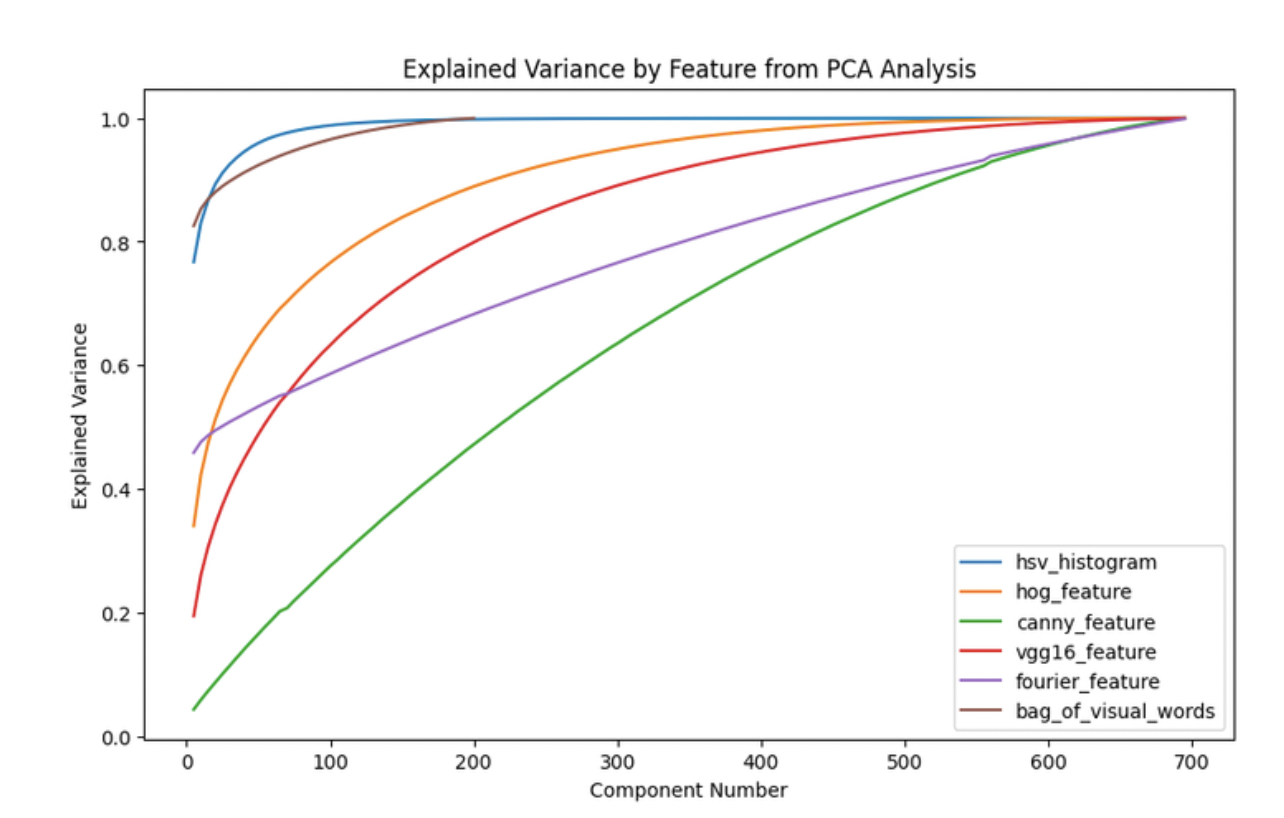
\includegraphics[width=0.8\textwidth]{PCA.png}
\caption{PCA plot of explained variance vs component number per feature. }
\label{fig:PCA}
\end{figure}

To identify the PCA number of components to use in our models, we utilize the number at the point of inflection instead of at the 90-95\% expected variance range. Table \ref{table:PCA} shows the explained variance at the point of inflection per feature. We make this decision to further reduce the number of components in our models. After the point of inflection, when there is a plateau, the expected variance does not increase significantly. Therefore, we reasonably conclude that utilizing the inflection point is sufficient for initial analysis. One exception to this rule is the Fourier feature which does not show a strong point of inflection. Given that we want to continue using this feature for the classification of edge frequencies, we chose an arbitrary number of components of 25. 

\begin{table}[h!]
    \centering
    \begin{tabular}{|l|c|c|}
        \hline
        \textbf{Feature} & \textbf{Explained Variance} & \textbf{Number of Component} \\
        \hline
        hsv\_histogram & 0.873 & 50 \\
        \hline
        hog\_feature & 0.692 & 100 \\
        \hline
        vgg16\_feature & 0.570 & 200 \\
        \hline
        fourier\_feature & 0.476 & 25 \\
        \hline
        bag\_of\_visual\_words & 0.764 & 40 \\
        \hline
    \end{tabular}
    \caption{Feature Analysis}
    \label{table:PCA}
\end{table}


\subsection{t-SNE Visualization}
t-distributed Stochastic Neighbor Embedding (tSNE) is run on the training dataset (10,786 images) per feature before PCA.

As shown in Figure \ref{fig:tsne}, HSV shows class differentiation between “forest” and “glacier” classes. We believe this is due to the different hues of a forest, mostly green, compared to those in glaciers, mostly white. HOG and Fourier differentiate between “street”/”forest” and “glacier”/”sea”. We believe this is due to commonalities they share in the directionality of their edge vectors. Forests and streets both contain more vertical edges than glaciers and horizons from the sea. VGG16 tSNE differentiates between classes most distinctly. There is some overlap between “street” and “building” classes possibly due to limited data present in the pre-training ImageNet database. Finally Canny and BOVW show none or limited class clustering. This suggests that they may not be as successful at classifying our images. We suspect this may be the case due to limited objects in our dataset.

Overall, tSNE gives insight into the classification ability of our features in a visual way. It gives us insight into what may be easily distinguishable vs cause confusion between our classes. We suspect that “buildings” and “street” may be incorrectly classified as one another as well as “glacier” and “mountain”, and “sea”.

\begin{figure*}[h!]
\centering
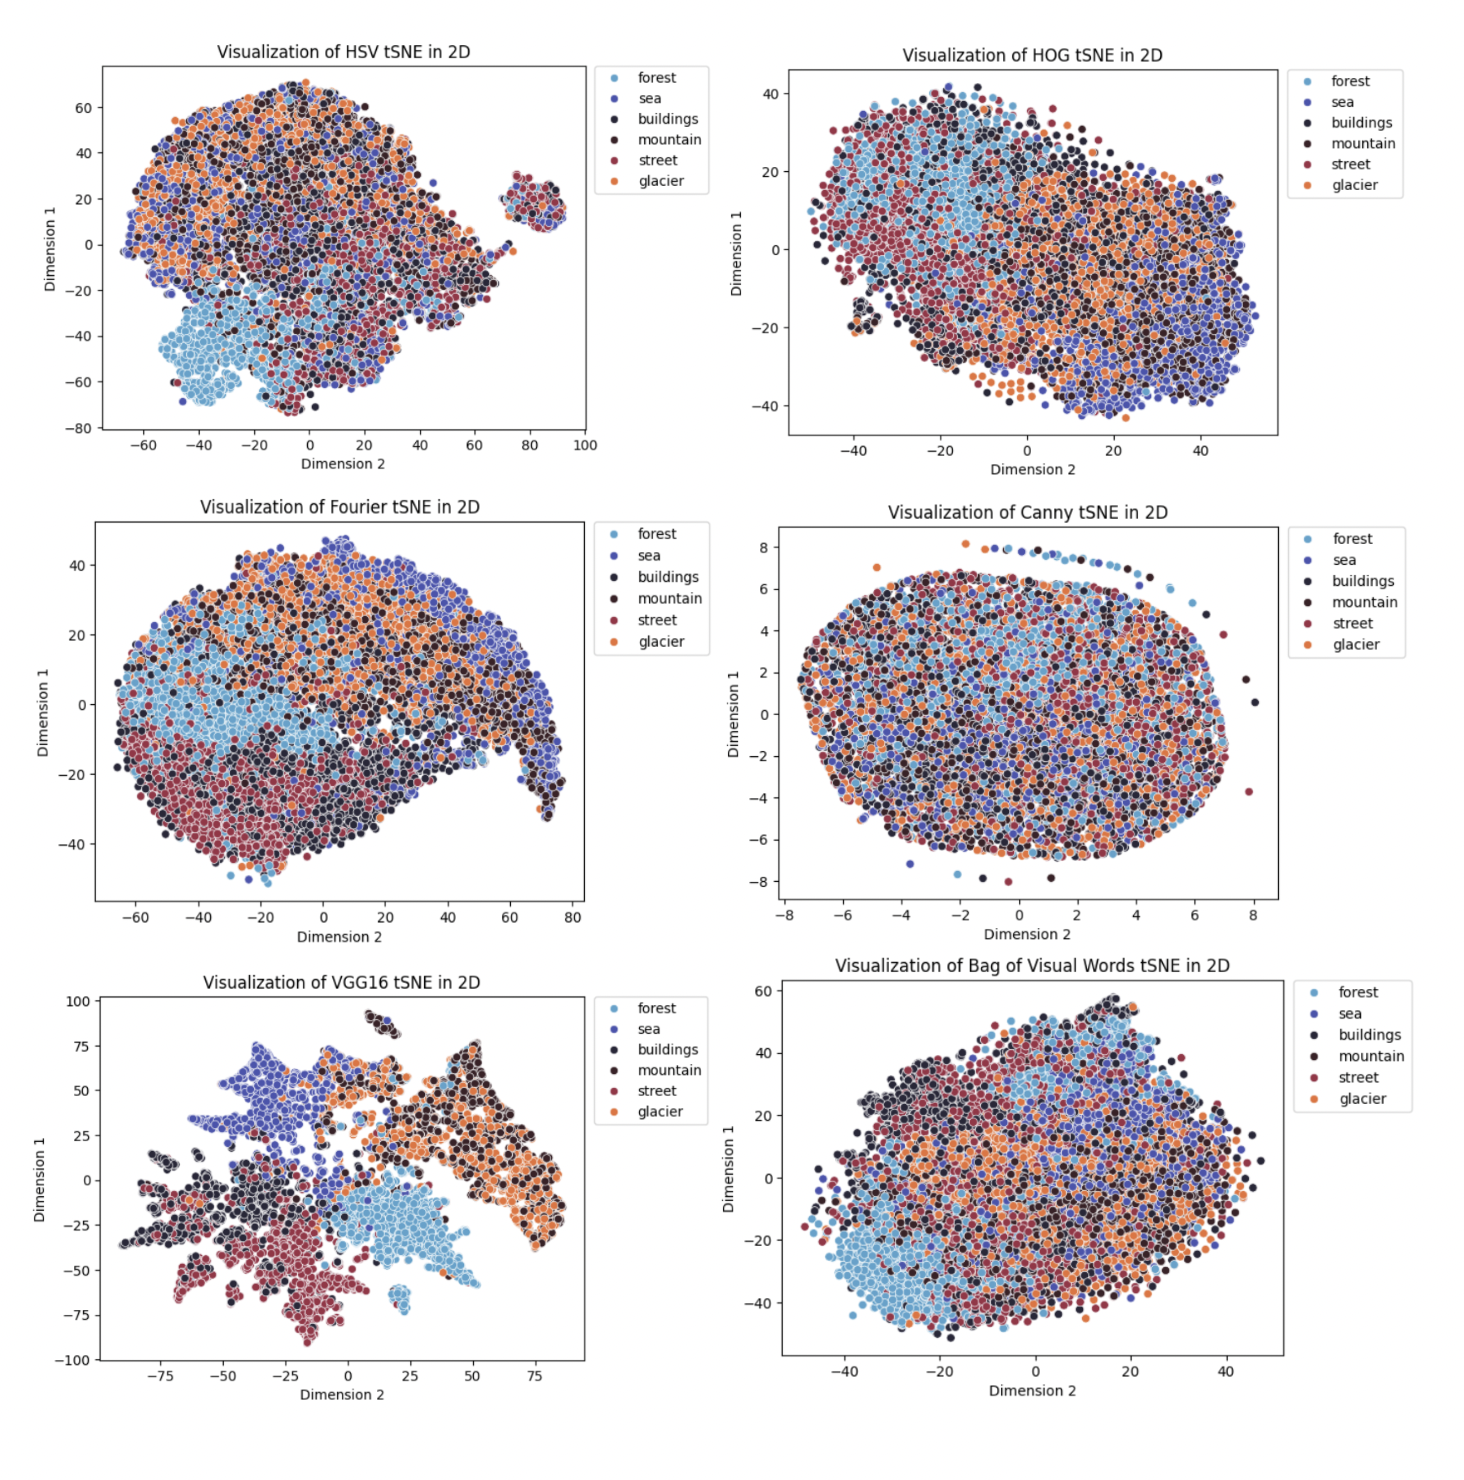
\includegraphics[width=0.8\textwidth]{tsne.png}
\caption{Scatter plot of 2-dimensional tSNE evaluation for HSV histogram, Histogram Of Gradient , Fourier transform, Canny edge detection, VGG16, and Bag Of Visual Words.
}
\label{fig:tsne}
\end{figure*}

\subsection{Lasso Regression}
Our baseline model is a logistic regression model with l1 regularization (max\_iter=100, C=0.1). We look at the feature importance of all features, including 1) mean RGB channels, 2) mean HSV channels, 3) HSV histograms, 4) Histogram of Oriented Gradient (HOG), 5) Bag of Visual Words (BOVW) , 6) Fourier Transform 7) pretrained VGG16 features. We drop the mean of RGB due to its low feature importance and keep all other six features in our model testing.

\section{Results}
In this section, we present various classifiers that we use, including logistic regression, support vector machine, and random forest. We discuss our approach for hyperparameter tuning to find the optimal parameters for each model. We show results on each classifier for all categories and discuss their strengths and weaknesses. 

\subsection{Hyperparameter Tuning}

\begin{table}[h!]
\centering
\begin{tabular}{|c|c|c|c|c|c|}
\hline
\textbf{Model} & \textbf{Parameter} & \textbf{Search Value} & \textbf{Best Value} & \textbf{Best F1 (val)} & \textbf{Search Time} \\
\hline
\multirow{3}{*}{LR} & ‘C’ & [0.01, 0.1, 1, 10] & 0.1 & \multirow{3}{*}{0.9250} & \multirow{3}{*}{3 min 10 sec} \\
\cline{2-4}
 & ‘penalty’ & ['l1', 'l2'] & l1 & & \\
\cline{2-4}
 & ‘max\_iter’ & [100, 200, 500] & 100 & & \\
\hline
\multirow{2}{*}{SVM} & ‘C’ & [0.1, 1, 3, 10] & 3 & \multirow{2}{*}{0.9188} & \multirow{2}{*}{2 min 12 sec} \\
\cline{2-4}
 & ‘kernel’ & ['linear', 'rbf'] & ‘rbf’ & & \\
\hline
\multirow{2}{*}{RF} & ‘n\_estimators’ & [100, 500] & 500 & \multirow{2}{*}{0.8990} & \multirow{2}{*}{7 min 1 sec} \\
\cline{2-4}
 & ‘max\_depth’ & [4, 6, 8, 10] & 10 & & \\
\hline
\end{tabular}
\caption{Hyperparameter tuning for logistic regression, support vector machine, and random forest models.}
\label{table:hyperparam}
\end{table}

After narrowing down the number of features through PCA, t-SNE and Lasso Regression, we conduct 40 experiments employing grid search with 5-fold cross-validation in the hyperparameter step. The optimal parameters are determined based on their F1 scores on the validation set. Table \ref{table:hyperparam} shows the parameters that we search, the total amount of time for the grid search, as well as the optimal hyperparameters for each model. 

\subsection{Model Results}
In table \ref{table:model_performance}, we note the top three models using the optimal hyperparameters. Logistic Regression (LR) attained the highest F1 score on the validation set, therefore, we pick it as our most accurate model. We also ran all three models in the test set, and Support Vector Machine (SVM) excelled with the best score.

\begin{table}[ht]
\centering
\begin{tabular}{|c|p{4cm}|p{2cm}|p{2cm}|p{2cm}|}
\hline
\textbf{Model} & \textbf{Best Params} & \textbf{f1(Train)} & \textbf{f1(Valid)} & \textbf{f1(Test)} \\
\hline
LR & ‘C’: 0.1, ‘penalty’: ‘l1’, ‘max\_iter’: 100 & 0.9432 & 0.9250 & 0.9191 \\
\hline
SVM & ‘C’: 3, ‘kernel’: ‘rbf’ & 0.9970 & 0.9188 & 0.9215 \\
\hline
RF & ‘N\_estimators’: 500, ‘max\_depth’: 10 & 0.9430 & 0.8990 & 0.8964 \\
\hline
\end{tabular}
\caption{Model Performance Comparison for Logistic Regression, Support Vector Machine, and Random Forest using their optimal parameters.}
\label{table:model_performance}
\end{table}


\subsection{Logistic Regression}
\textbf{Best Parameters: 'C' = 0.1, 'penalty' = 'l1', 'max\_iter' = 100.} \\
The model selects a lower ‘C’, the inverse of the regularization parameter, suggesting that a moderate amount of regularization could help prevent overfitting. The preference for the ‘l1’ penalty over ‘l2’ indicates a need to further reduce dimensions for improved model performance. The ‘max\_iter’ parameter set at 100 is standard and implies that additional training might lead to overfitting.

The logistic regression model achieved the highest F1 score on the validation set is 0.9250, with training and test F1 scores of 0.9432 and 0.9191, respectively. It is our strongest model. The consistency of the F1 scores across training, validation, and test sets demonstrates good generalization.

\subsection{Support Vector Machine}
\textbf{Best Parameters: ‘C’ = 3, ‘kernel’ = ‘rbf’.}\\
The relatively high ‘C’ value in the SVM model suggests that a higher penalty on errors is necessary for better model performance, with the trade-off having a lower margin, which may lead to over-fitting. The kernel, a function for mapping data into a higher-dimensional space, is set to ‘rbf’, given the nonlinearity in our image data.

The support vector machine model exhibited excellent performance on the training set (F1 score of 0.9970) but experienced a slight decline in the validation and test sets (0.9188 and 0.9215, respectively). This might indicate some overfitting to the training data, potentially attributed to the higher ‘C’ value.

\subsection{Random Forest}
\textbf{Best Parameters: ‘N\_estimators’ = 500, ‘max\_depth’ = 10. }\\
'N\_estimators' represents the number of trees in the forest, and 'max\_depth' determines the maximum depth of these trees. The selection of 500 trees with a maximum depth of 10 suggests a requirement for a more complex model in our classification task but also poses a risk of over-fitting.

The Random forest model does not significantly outperform the simpler Logistic Regression model, with F1 scores of 0.9430, 0.8990, and 0.8964 on the training, validation, and test sets, respectively. This suggests that the complexity of Random Forest may not provide substantial benefits over the more straightforward Logistic Regression model.

Overall, all three models demonstrated strong capability to effectively differentiate urban scenes from natural landscapes. The Logistic Regression model showed the best balance between performance and generalization. 

\subsection{Inaccurate Predictions}
To enhance the model, we analyze the inaccurate predictions using the confusion matrix (Figure \ref{fig:confusion_matrix}), as well as the precision, recall and f1 score for each category (Figure: \ref{fig:classification}). We observe that most misclassifications occur between glaciers and mountains, as well as streets and buildings. 

\begin{figure}[h!]
    \centering
    \begin{minipage}[b]{0.48\textwidth}
        \centering
        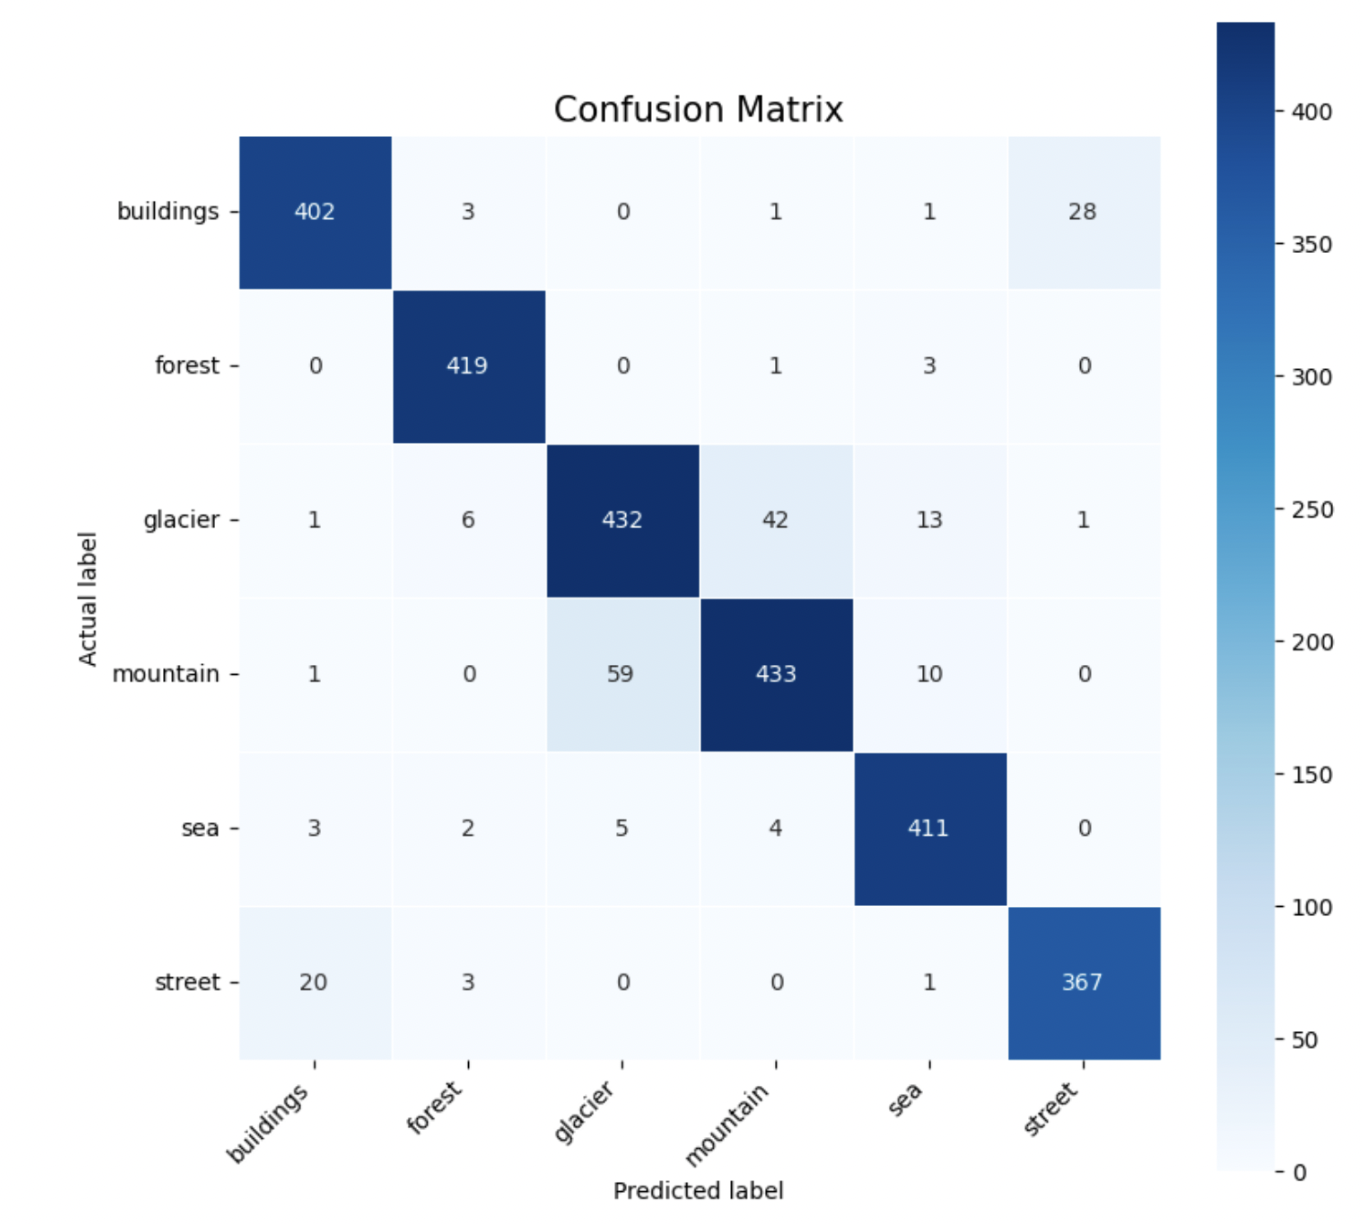
\includegraphics[width=\textwidth]{confusion_matrix.png}
        \caption{Confusion matrix for Logistic Regression.}
        \label{fig:confusion_matrix}
    \end{minipage}\hfill
    \begin{minipage}[b]{0.48\textwidth}
        \centering
        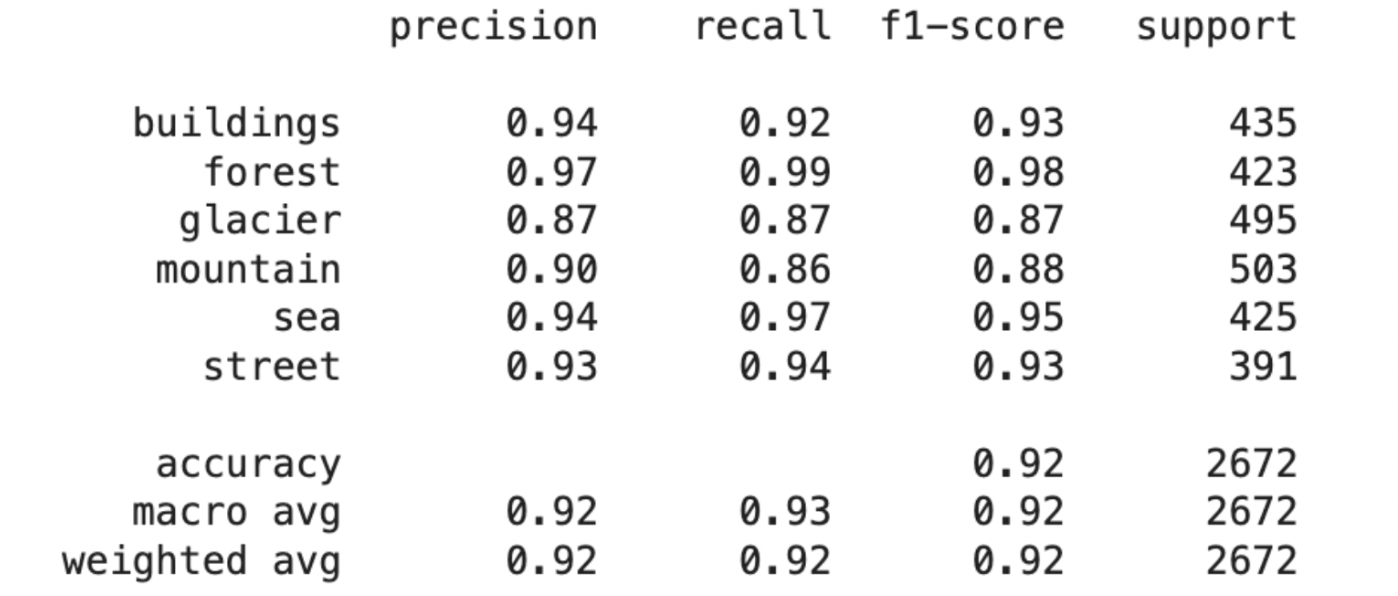
\includegraphics[width=\textwidth]{classification.png}
        \caption{Precision, Recall, and F1 Score for all categories for Logistic Regression.}
        \label{fig:classification}
    \end{minipage}
\end{figure}


We generated sample images of these inaccurate predictions, as displayed in Figure \ref{inaccurate_images}. The image on the left shows a snow-covered mountain with challenging lighting conditions, suggesting that white balancing during the preprocessing phase may help with natural scenes. The image on the right is a street-like scene with a single large building. This observation leads us to consider that counting the number of objects could be a useful feature for enhancing accuracy, as the 'buildings' label typically presents one or a few buildings, whereas 'streets' are characterized by multiple structures.

\begin{figure*}[h!]
\centering
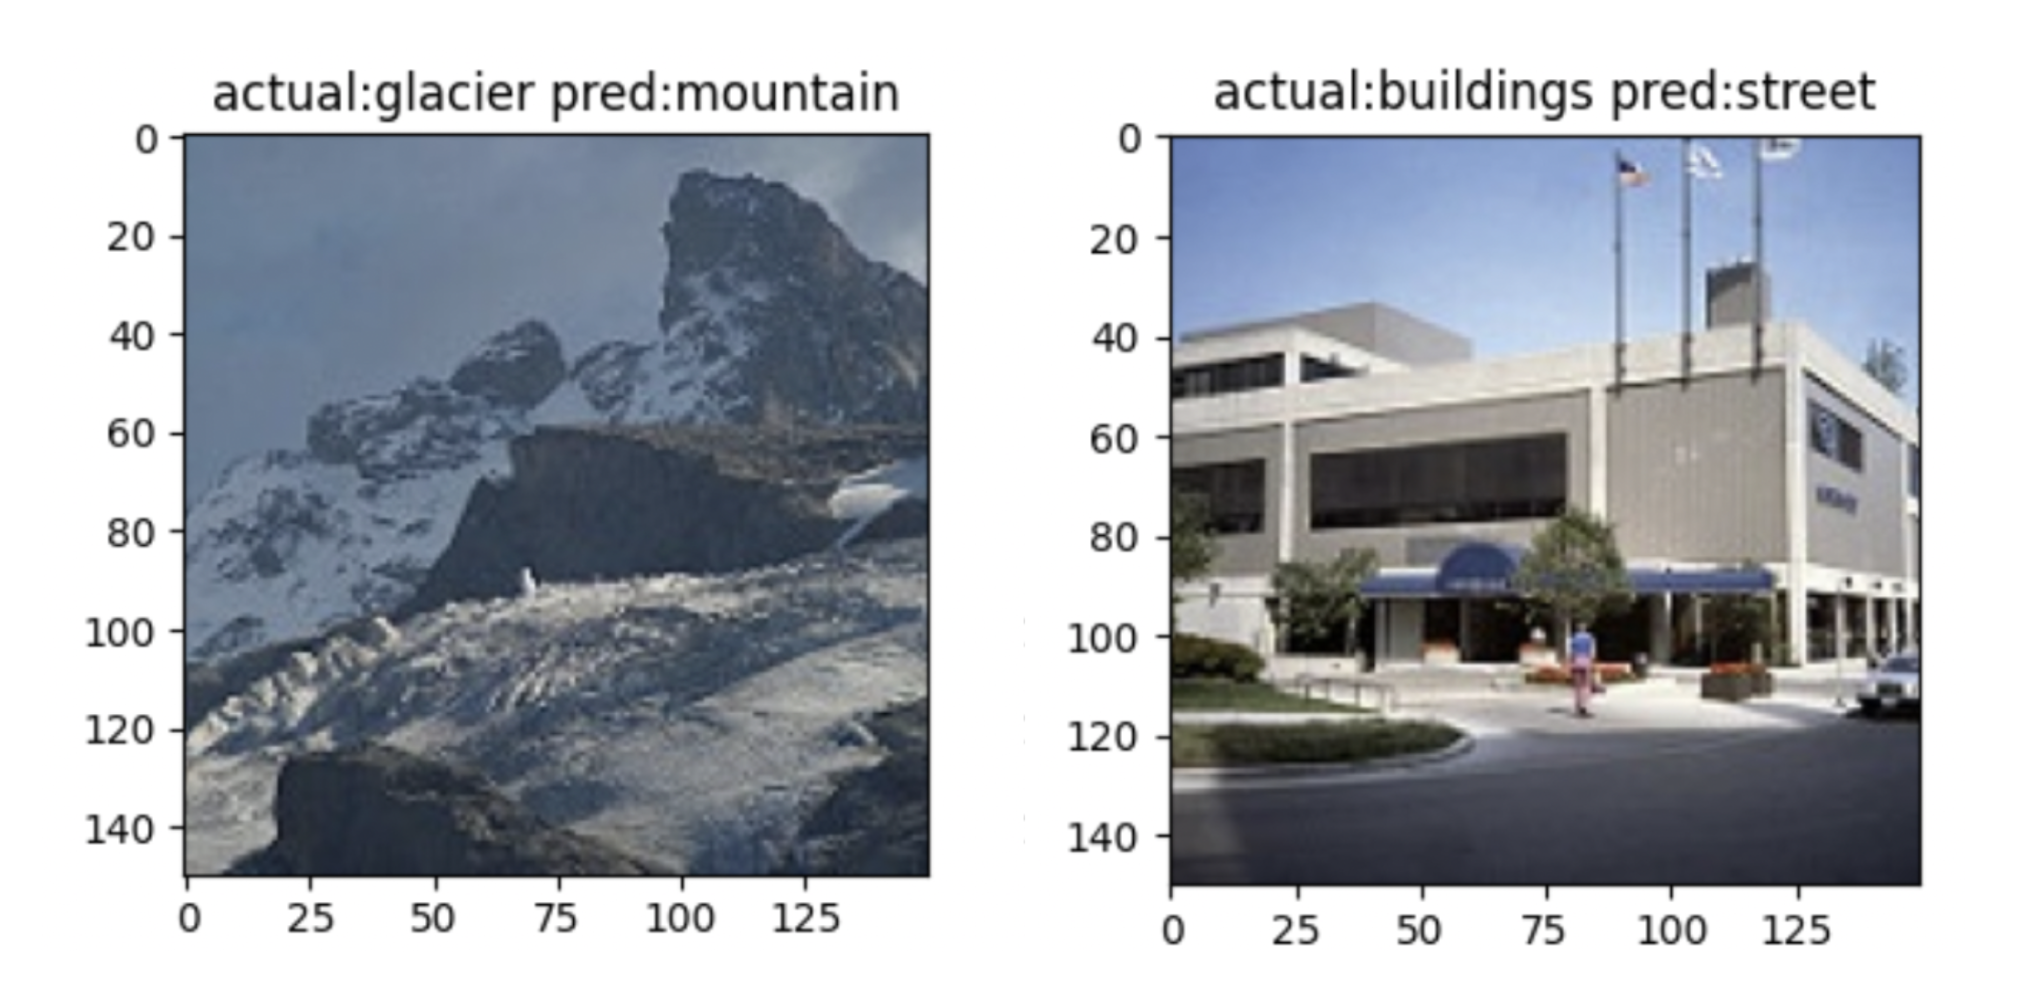
\includegraphics[width=0.7\textwidth]{inaccurate_images.png}
\caption{Sample images for misclassification.}
\label{fig:inaccurate_images}
\end{figure*}


\section{Generalizability}
We put generalizability as a priority during our model training process. Following common practice, we split the training set into 80\% training, and 20\% validation, and leave the test set as it is. Our final split across the train, validation, and test set is 66\%, 16\% and 18\%. We use our validation set only for model selection and only use the test set to demonstrate results when three best models are selected.

Given our image dataset size, we understand that we need to reduce dimension significantly to prevent overfitting. In the PCA step, we make the choice of picking the point of inflection on the explain variance graph for each feature, over-picking the number of components that achieved 90-95\%, which would lead to 10x more parameters. This decision helps us minimize overfitting issues in all three models.

During hyperparameter tuning, we also use grid search with 5 fold cross validation to identify the optimal parameters using macro F1-score across six categories, adding another layer of stability in the models. In Table \ref{table:model_performance}, the consistency between train, validation and test sets also suggest generalizability in our prediction.

\section{Efficiency vs. Accuracy}
In table \ref{table: time}, we note the model training time employing 5-fold cross-validation, as well the inference time on train and validation sets for all three models. Our experiment is performed on Google Colab Pro with a CPU configuration of Intel(R) Xeon(R) CPU @ 2.20GHz and 40 GB RAM. 

Overall, Logistic Regression is notably efficient in both training and inference phases, demonstrating very low latency in predictions across all datasets. Support Vector Machine, despite its reasonable training time, has significantly longer inference times, which could be a drawback in scenarios requiring quick responses. 

\begin{table}[h!]
    \centering
    \begin{tabular}{|p{3cm}|p{3cm}|p{3cm}|p{3cm}|}
        \hline
        \textbf{Model} & \textbf{Model Train Time (CV)} & \textbf{Inference Time (Train)} & \textbf{Inference Time (Valid)} \\
        \hline
        LR & 3 min 10 sec & 25.3 ms & 6.38 ms \\
        \hline
        SVM & 2 min 12 sec & 42.8 s & 10.5 s \\
        \hline
        RF & 7 min 1 s & 1.14 s & 284 ms \\
        \hline
    \end{tabular}
    \caption{Training and inference time for logistic regression, support vector machine and random forest model.}
    \label{table: time}
\end{table}


\subsection{Feature Contribution}
To further understand feature contribution and enhance model efficiency, we reduce each feature in the full model to evaluate the balance between performance and training time. We also exclusively test a model using VGG16 alone, given its prominent performance.

As observed in Table \ref{table:feature_combination}, we note that the Logistic Regression model with VGG16 alone yields similar results on the validation set (0.9156 vs. 0.9250 F1 score), while cutting the training time in half (29.63 sec to 13.01 sec). Eliminating any other simple feature individually does not impact the model performance or result in time saving. But the model with four simple features without VGG16 can also achieve 0.82 F1 Score, suggesting our effectiveness in extracting information from simple features.

\begin{table}[h!]
    \centering
    \begin{tabular}{|p{4cm}|c|c|c|}
        \hline
        \multicolumn{1}{|c|}{\textbf{LR Model}} & \textbf{f1\_macro (Train)} & \textbf{f1\_macro (Valid)} & \textbf{Train Time (each fold)} \\
        \hline
        full model & 0.9432 & 0.9250 & 29.63 sec \\
        \hline
        VGG16 only & 0.9287 & 0.9156 & 13.01 sec \\
        \hline
        w/o HSV & 0.9386 & 0.9178 & 25.53 sec \\
        \hline
        w/o HOG & 0.9358 & 0.9251 & 29.51 sec \\
        \hline
        w/o Fourier & 0.9421 & 0.9257 & 28.10 sec \\
        \hline
        w/o VGG16 & 0.8375 & 0.8210 & 14.43 sec \\
        \hline
        w/o BOVW & 0.9402 & 0.9238 & 26.64 sec \\
        \hline
    \end{tabular}
    \caption{Model results for experiments on various features combination in logistic regression model. }
    \label{table:feature_combination}
\end{table}


\section{Conclusion}
In summary, we chose the HSV histogram, Fourier Transformation, Bag of Visual Words, Histogram of Oriented Gradients, and the pretrained VGG16 embeddings as our final features. The logistic regression with L1 regularization and a C parameter of 0.1 emerges as our most accurate and generalizable model. This is determined based on its superior performance in the validation set, achieving a 0.92 F1 Score. It is also our most efficient model based on its inference time. VGG16 is a powerful network for our classification task, while our work on feature extraction on simple features also captures the essential visual aspects of our images.

\bibliographystyle{plain}
\bibliography{sample}

\end{document}